\section{Technical background}\label{tech-oview}
Short intro about this section - its about giving the reader a detailed overview of the technology used, to showcase that we know what we talk about and to demonstrate that these technologies fit into answering the research question.

\subsection{PID types and naming scheme}\label{pid-types}
Over the years, different kinds of PIDs have emerged. The most widely used PID types are Handle (first major PID type introduced 
in 1994), Digital Object Identifier (DOI), Persistent URL (PURL), Uniform Resource Name (URN) and 
Archival Resource Key (ARK) \cite{pid-oview, odin, hdl}. For our PoC described in section \ref{pid-poc}, we have looked into Handle, DOI and URN in detail. For a technical overview of the aforementioned PID types we refer to the research done by Karakannas \cite{icn-bd}. 

The most widely used PID types make use of the same hierarchical naming scheme, which starts with a PID type identifier
 such as \texttt{"urn"}, \texttt{"handle"} or \texttt{"doi"}, followed by some kind of delimiter. The PID type identifier is usually embedded in the URL of the PID resolver naming authority 
such as \texttt{"http://hdl.handle.net/"} for resolving Handle PIDs, \texttt{"https://doi.pangaea.de/"} for resolving DOI PIDs or \texttt{"http://resolver.kb.nl/resolve?urn="} for resolving URN PIDs, followed by the PID of the digital object. This means that PIDs are usually associated with a resolver via a URL \cite{ids, icn-bd}. A PID web resolver redirects to the location of the digital object.
After the first delimiter, the naming authority is defined (this can be seen as a prefix of a digital object), followed again 
by some kind of delimiter. At last there is a Namespace Specific String, which is the identity of a digital object within the naming authority which syntax depends on the naming
authority. Table \ref{tab:pid} below shows an overview of the mentioned PID types. 
%A more in-depth description of PIDs can be found in \cite{icn-bd} and \cite{pid-oview}.

%For a more in-depth description of PIDs we refer to \cite{icn-bd} and \cite{pid-oview}.

\begin {table}[H]
\caption {Hierarchical scheme of PID standards \cite{icn-bd}.} \label{tab:pid} 
\begin{center}
\scalebox{0.82}{%
  \begin{tabular}{| c | c | c | c | c | c | }
    \hline
    \textbf{PID types} & \textbf{PID Type Identifier} & \textbf{Delimiter} & \textbf{Authority} & \textbf{Delimiter} & \textbf{Name} \\ \hline
    \textbf{URN} & urn & : & \textless NID\textgreater & : & \textless NSS\textgreater \\ \hline
    \textbf{Handle} & hdl & : & \textless Handle Naming Authority\textgreater & / & \textless Handle Local Name\textgreater \\ \hline
    \textbf{DOI} & doi & : & 10.\textless Naming Authority\textgreater & / & \textless doi name syntax\textgreater \\ \hline
  \end{tabular}}
\end{center}
\end {table}


%Talk about how DOI is interoperable within Handle? \textgreater Yes. The PID type providers we came accross make use of XML metadata for URN (Duth Royal Library) etc.

\subsubsection{URN}
%Metadata in XML, so you need XML parser etc.. for using metadata info in NDN name.
The URN PID standard was first introduced in RFC 1737. It is based on the URI syntax and its syntax is shown in figure \ref{tab:pid}. The \texttt{\textless NID\textgreater} part is the Namespace Identifier, this identifies the namespace or to be more specific the authority that publishes the specific URN.
The syntax of the Namespace Specific String part \texttt{\textless NSS\textgreater} depends on on the authority identified by the \texttt{\textless NID\textgreater}. This part can be used from the authority for further delegation to sub-authorities \cite{icn-bd}.

The Dutch Royal Library uses URNs and maintains a web accessed URN resolver that can resolve a URN to a URL, which can be then used to retrieve the digital object. For example the following URL \url{http://resolver.kb.nl/resolve?urn=anp:1938:10:01:2:mpeg21}. 
They store the metadata of a digital object in an XML scheme, which can be requested in a API call \cite{kb-urn}. The metadata can be parsed to be used in an NDN name to fill in possible naming gaps as discussed by Olschanowsky et. al. \cite{ndn-clim} highlighted in section \ref{introduction-related-work}. This applies to all upcoming PID types discussed in this section.

\subsubsection{Handle}
The Handle system was developed by Bob Kahn at the CNRI in 1994, and currently administered and maintained by the DONA Foundation. The CNRI is the root server of the Handle System and maintains all the Handle Naming Authorities, where each Handle Naming Authority can establish its own resolution infrastructure. This makes it possible for the Global Handle System to delegate queries for Handle resolution. 
Its main functionalities are specified in RFC 3650. In 2015 it supported, on average, 68 million resolution requests per month where the largest single user being the Digital Object Identifier (DOI) system, which will be discussed below in section \ref{doi} \cite{hdl-us}. 

The Handle syntax is shown in figure \ref{tab:pid}. The Handling Name Authority part of the syntax is a prefix that it is assigned by the Global Handle
Service and its hierarchical structure is similar to DNS domain names. The Handle Naming Authority is a sequence of decimals that are separated by the
dot(".") character, for example one can get assigned the prefix \texttt{20.4000.581}. 
The slash("/") delimiter separates the Handle Naming Authority from the Local Handle Name syntax. In this part a PID provider can specify the identity of a digital object within the Handling Name Authority it gets assigned. 
The only limitation for the Handle Local Name syntax is that it can only contain printable characters from Unicode's
UCS-2 character set.

The path of a Handle PID is read from the left to the right and the dot(".") character is defines the hierarchy of the Naming Authorities. The naming hierarchy
does not imply any technical implication. Which means that the Handle Naming Authority \texttt{"20.5000.481"} can be independent of the Handle Naming Authority \texttt{"20.5000"} \cite{icn-bd}.

For Handles, a web accessed URN resolver can also be used to resolve a Handle PID to a URL. For example the following URL, \texttt{http://hdl.handle.net/20.5000.481/data/objects/object1}. The Handle system makes use of the restful JSON API for retrieving metadata \cite{hdl-api}.

%Metadata in JSON, so you need JSON parser etc.. for using metadata info in NDN name.

\subsubsection{DOI}\label{doi}
%Metadata in JSON, so you need JSON parser etc.. for using metadata info in NDN name.
DOI makes used of the Handle system as described earlier. The Handle System was selected for the resolution task within the DOI system because it matched the resolution requirements identified for the DOI concept \cite{doi-found}. It is managed and
controlled by the International DOI Foundation (IDF). The DOI system has been assigned the \texttt{<Handle Naming Authority>} value 10 in the Global Handle System as shown in table \ref{tab:pid}. Just like Handle, it uses a slash ("/") delimiter to separate the PID authority from the PID name.

The DOI system is mostly an administrative framework for assuring common practices and standards for publishing and maintaining handles between the Registration Agencies (RAs). An RA is an organization or institution which ensures specific quality standards in order to participate in the DOI project and is responsible for assigning DOIs to digital objects. 
The \texttt{<doi name syntax>} part identifies an object within the DOI naming authority. 

The DOI Resolver is the apex in the hierarchy and it can resolve any RAs' DOI to a URL from which the digital object can be retrieved \cite{icn-bd}. 
%This also achieves resolving DOIs to the digital object by a web accessed resolver.
This makes the resolution of a DOI to the digital object also achievable by a web accessed resolver. The PANGAEA information system aimed at archiving, publishing and distributing georeferenced data from earth system research uses DOI \cite{pang}. A DOI URL used by PANGAEA is for example \texttt{https://doi.org/10.1594/PANGAEA.339110}.
Furthermore, in the DOI system metadata is available in many formats, including Bibtex, Citeproc-JSON, RDF as well as XML and JSON \cite{doi-met}. It depends on the PID provider which format to choose.

%\subsubsection{ARK}
%ARK is also one of the most widely used PID types used for persistent identification of digital objects. The ARK system was created in 2001 by the US National Library of Medicine and is currently maintained by the California Digital Library (CDL) \cite{ark-typ}. Its syntax is shown in table \ref{tab:pid}. The Name Assigning Authority Number\texttt{<NAAN>} part identifies the Naming Assigning Authority (NAA) that assigned the specific ARK. The NAAN is a string and consists of five to nine decimals that uniquely identify each NAAN.

%The \texttt{<Name>} part in the ARK syntax identifies the digital object, which is unique among the NAAN scope. The \texttt{<Name>} part consists of a string, which is composed of printable ASCII characters and should be less than 128 bytes in length.

%The \texttt{[<Qualifier>]} part is an optional parameter of the ARK syntax and specifies a variant of a digital object. It can be added by appending a dot(".") character after the \texttt{<Name>} part. 

%Resolving ARKs is like the aforementioned PID types also achieved by a web accessed resolver called the Naming Mapping Authority (NMAH). 
%Each NAA utilizes its own NMAH that resolves the ARK to a URL, which is used for retrieving the digital object \cite{icn-bd}.

%The Name-to-Thing resolver (N2T) is an example of a ARK web resolver. It was originally designed for global resolution of ARK identifiers only, but is nowadays general enough to apply to identifier schemes from any PID type. An example of a ARK URL, which is resolved by the N2T resolver is \texttt{https://n2t.net/ark:/12345/fk1234} \cite{n2t}. To access metadata, a question mark ("?") has to be appended at the end of the URL where the API then returns metadata in the Electronic Resource Citation (ERC) format \cite{ark-erc}. 

%\subsubsection{PURL}
%PURL is yet another PID type that was developed from the Online Computer Library Center (OCLC). The PURL naming syntax is shown in table \ref{tab:pid}. The \texttt{<protocol>} part specifies the protocol used to access to resolver of the PURL and the  \texttt{<resolver address>} part is the location of the resolver from which the digital object specified in the \texttt{<name>} field can be resolved.

%Basically, a PURL is a URL that points to a resolver that does the mapping
%between the \texttt{<name>} part and the actual URL from which the digital object can be
%retrieved instead of pointing directly to the location from which the digital object can be retrieved \cite{icn-bd}.

%The Federal Depository Library Program (FDLP) is a U.S. government program which utilizes the use of PURL for uniquely identifying federal government publications and making them publicly available \cite{purl-fdlp}. An example link that their PURL resolver resolves to its location is \texttt{https://purl.fdlp.gov/GPO/gpo121591}.
%Worth mentioning is that no additional metadata is used in PURLs \cite{eudat-pid}.




%%% KAAS


\subsection{NDN}
\label{overview-ndn}
% Brief overview of technical components, such as; PIT, CS, FIB, strategies (cache, replacement, forwarding)
In NDN the content can be retrieved from any source that has the named data. Data is named in NDN by typically a hierarchical name, in which a prefix can be used to match a specific tree of an organization. \todo{Find better illustration for NDN name} Figure \ref{fig:ndn_name}, taken from Jacobson et al. \cite{jacobson2009networking} is an example of an NDN named video file. This named data object is made available under the prefix \texttt{/parc.com}, which is the globally-routable name. This globally-routable name is in practice assigned by an organization (operations similar to DNS allocation of today). All data under this prefix are automatically published and available in NDN. These can then be downloaded from the original publisher, a repository, a router cache or a neighboring peer in a local network. NDN can be used as an overlay on any type of network e.g. TCP/IP, but also Bluetooth. All content can be authenticated by the use of integrity checks to ensure untained copies of the data. Efficient distribution is achieved by caching at intermediary hops in the NDN network. These hops can be NDN routers, but also cellphones and laptops. This distributed nature of NDN provides parallel transfers such as bulk data distribution and thus collaboration simultaneously on the same datasets, such as climate change data.

\begin{figure}[H]
\centering
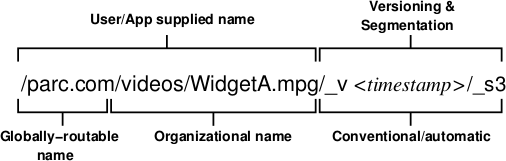
\includegraphics[width=\columnwidth/2]{Images/ndn_name.png}
\caption{NDN name scheme example.}
\label{fig:ndn_name}
\end{figure}

The receiving end in NDN is in control of communication. Two distinct packets are used to drive communication; interest and data packets. In order to query for data names in the NDN network, the interest packet is used. When this interest packet is received by a node in the NDN network that has the data, a data packet is returned. This data packets is send back over the same route as the interest packet was sent, resulting in symmetric forwarding. As discussed earlier, data may be cached on the intermediary hops in the NDN network.

NDN has an advantages over TCP/IP, it's able to use multiple paths and unlike TCP/IP it's able to handle loops at the forwarding layer. A loop-free topology is realized by inserting a nonce in every interest packet which allows to identify duplicate interests for named data, allowing multiple paths to be used which could increase throughput efficiency. Information about paths in the network are maintained in a layer called the strategy layer. This layer keeps track of two-way traffic and changes local forwarding decisions based on traffic observations. A face in NDN holds a connection to a forwarder, which could be of any class of the underlay (e.g. TCP/IP, Bluetooth or any other supported underlay).

The NDN packet forwarding engine is composed out of three data structures; The FIB, CS and PIT. The FIB is used to forward interest packets towards potential sources(s) of matching data. The FIB allows a list of outgoing faces towards a certain prefixes. In contrast to an IP FIB, a list for a single destination is not allowed due to network loop problems. The behavior of the forwarding can be changed by using different forwarding strategies. Before an interest packet is send out to the FIB it is first stored in the PIT along with the requesting face. An interest packet will remain in the PIT until a user defined timeout is reached, or when a matching data packet has returned from a source. The prefix and requesting face in the PIT define a return path back to the requester at each hop, this is referred to as the breadcrumbs path. The CS acts as the cache in NDN, which is used to provide the distributed property in NDN. This cache also has strategies, one for evicting data objects from the cache and one for stashing data objects in the cache.

As described in section \ref{overview-ndn} there are two kinds of caching strategies; a caching decision and a cache replacement strategy. A caching decision strategy is used to determine in which router along the reverse path of an interest packet will cache the data \cite{koulouzis2018information}. Below are the most well-known caching decision strategies are listed.

\begin{itemize}
    \item Leave copy everywhere; used to cache data object packets along each hop in the NDN path.
    \item Leave copy down; used only by the first router in the NDN path after either the original producer or an NDN cache.
    \item Leaving copies with probability; used to cache those data objects with the probability of 1/(hop count).
    \item Leaving copies with uniform probability; used to cache data objects with uniform probability.
\end{itemize}

A cache replacement strategy is used to determine which data objects to evict from the cache in order to make room for new data objects. Below are the most well-known caching eviction strategies are listed.
\begin{itemize}
    \item First in first out; used to evict the first data object that was inserted from the cache.
    \item Random replacement; used to evict random data objects from the cache.
    \item Least recently used; used to evict the least recently used data object from the cache.
    \item Least frequently used; used to evict the least frequently used data object from the cache.
\end{itemize}

The information stored in the PIT and FIB can be used to determine how to forward in interest packet out to one or more faces. These strategies are meant to give adaptive decisions based on network conditions. Below are the most well-known forward strategies are listed.
\begin{itemize}
    \item Flooding; used to forward received interest packets towards every face, excluding the face the interest was received from.
    \item Best-route with caching; used to calculate the best path with Dijkstra's algorithm (least amount of hops) to reach a data object cache.
    \item Best-route without caching; used to only satisfy interest packets towards the original data publishers, thus excluding intermediary caches along the NDN path. 
\end{itemize}

\subsection{McCabe}
\label{overview-mccabe}
% Describe his method in more detail, explain adaptions towards ndn, if applicable.
% Add diagram to description, to illustrate the flow of the train of thought
% discuss RMA from book
As briefly described in section \ref{introduction-related-work}, McCabe's book "Network Analysis, Architecture, and Design" \cite{mccabe2010network} is about applying a systems methodology approach towards network design. McCabe's approach consists out of three core phases; analysis, architecture and design. These phases in McCabe are describe how to make technology and topology decisions in a network. These decisions are guided based on inputs for the three core phases, the initial input can be from users and/or from network metrics. Consecutive processes use the output of previous processes as input, thus these processes that are interconnected. In this section we will describe McCabe's method in more detail.

In figure \ref{fig:mccabe-process} the three core phases are illustrated in \textit{italic} while the processes are in normal text. In order to highlight the core phases by name they are \underline{underlined} in the figure. The first phase (analysis) has as goal to understand the network and potential problems in terms of performance and efficiency in order to determine network requirements. This is done by developing sets of problem statements and objectives that describe what the target network should address. Therefore, historical data from network management (monitoring), requirements gathered from the network users, staff and management are included in the analysis phase. Furthermore, these metrics are then compared to the relationships between users, applications, devices and other networks in order to determine if requirements match with the user and network expectations. The second and third phase (architecture and design) uses the output of the first phase to establish a high-level design of the network. This network design determines which technology and topology choices are justified to improve the network requirements established in the first phase. The fourth process is implementing the design, test if requirements are met and finally accept the implementation. These phases are intended to be iterative and by no means define a final architecture design. This is due to the fact that requirements, technology and user behaviour can change and with that the network design.

\begin{figure}[H]
\centering
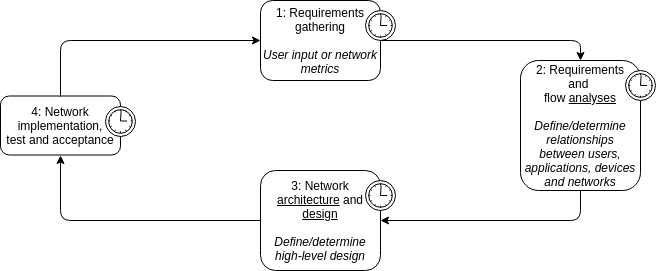
\includegraphics[width=\columnwidth]{Images/mccabe-process.png}
\caption{Cyclic and iterative nature of McCabe's processes and phases.}
\label{fig:mccabe-process}
\end{figure}

\subsection{TOSCA}
\label{overview-tosca}
% Why use it, why did we use it? Are there alternatives? Compare them shortly - if needed
% Highlight popularity, Google, RedHat, Canonical, etc. - to emphasize that TOSCA won't go away soon, but keeps growing
%Describe DRIP, OpenStack and an orchestrator in general
OASIS, an organization which is a global nonprofit consortium that works on open-standards, published the first TOSCA standard in 2014. The TOSCA standard is meant to standardize data modeling for cloud orchestration environments and applications. The latest version 1.1 standard \cite{tosca-standard}, was released in 2018. In this section we will highlight the important features of TOSCA, relevant to our research scope. Section \ref{method-planning} will merge TOSCA with McCabe's method (section \ref{overview-mccabe}).

Portability and automated management of enterprise IT infrastructures are major concerns. Infrastructures may need to run on heterogeneous components due to application needs. Having different descriptions of deployment and management for each environment complicates an infrastructure. This challenge introduces new requirements and concepts for deployment, configuration, operation and termination of components that make up an entire infrastructure. TOSCA provides a method to describe these components in generic modeling templates. In which an orchestrator can be used to implement these descriptions. Thus, TOSCA provides a single description for an entire infrastructure, which is then implemented by an orchestrator. This results into a portable (can be run by any orchestrator that understands TOSCA) and automated (implementations done by orchestrator) method of infrastructure management. This allows interoperability and reusability of TOSCA descriptions on different cloud providers. Seaclouds\footnote{\url{http://www.seaclouds-project.eu/}} (EU FP7 funded project), not to be confused with SeaDataCloud, is already managing infrastructures based on TOSCA. Google, Red Hat, Canonical and IBM are also involved with the development of TOSCA, signifying that broader adoption may follow in the future.

TOSCA descriptions consist out of the following core components; nodes, relationships and interfaces. Nodes can be a host, container or VM and are connected to each other through relationships such as dependsOn, hostedOn and connectsTo. These relationships can be used to describe that a VM is 'hosted on' a host (e.g. a bare metal machine). Or that a set of containers 'depend on' each other for functionality. Such as a containerized web application that requires a database, facilitated by another container. Interfaces are used as hooks to trigger actions, these actions are create, configure, start, stop or delete. These hooks can be triggered to e.g. configure and create containers, stop or start a service or do system maintenance such as delete artifacts after a service is stopped. Interfaces are used to control the life cycle of a component 

\subsection{Virtualization}
\label{overview-virtualization}
Virtualization is part of modern day infrastructures. It provides more efficient use of resources and flexibility because multiple VMs and containers can be deployed on any host that support them. VMs are complete operating systems that run in complete isolation from its host. Containers on the other hand share the kernel of its host and offer user-space isolation, which is relatively less isolation when compared to a VM. However, containers are more resource friendly than VMs in terms of needed compute power and disk space. This section will briefly describe these two forms of virtualization.

Cloud providers such as Amazon provide easy access to compute resources, one way to access these resources is by deploying a VM on their platform. Resources can be added or removed via management interfaces or API's. This allows an infrastructure, that runs on the Amazon platform, to flexibly scale in or out. Containers offer the ability to package software components together with all dependencies (e.g. libraries and binaries), such a package is called a container image. Docker is a popular platform to build and manage container-based virtualization. Once a Docker image is built it can be distributed through so-called Docker registries, such as Docker Hub\footnote{\url{https://hub.docker.com/}}. Kubernetes\footnote{\url{https://kubernetes.io/}} can be used to automate application deployment, scaling, and management of containers. In Kubernetes a container is called a pod, this may be a Docker container. These Kubernetes pods can be deployed in a cluster of Kubernetes nodes, spanning through e.g. different data centers. This offers great flexibility by packaging an application in a pod and then scale the application in or out through different data centers with Kubernetes. Kubernetes also offers availability features, such as automatically restart a pod when a crash occurs or load balance requests by using different pods in e.g. a round-robin fashion.

%\subsubsection{Docker}
%What is it, why use it, why do we use it and how?

%\subsubsection{Kubernetes}
%What is it, why use it, why do we use it and how?